\chapter{Screens, menu and buttons}\label{ScreensMenuButtons}

What you get is what you see. A bunch of screens in multiple tabs. What you see is not exactly what you get in terms of test patters.
To understand what you get you must first understand what you see. This chapter is all about that. Step by step all screen, all fields
and all buttons get explained.

There might be small deviations in the images here compared to the actual program. Changes in the program are not always immediate
reflected in the documentation.

The main form (and up to now the only form) is using several tabs for configuration and creating test patterns. Each tab is
a screen on its own right and needs an explanation. The organisation of the tabs and this explanation is from the more detailed
to the more global subjects. Where the `Test Pattern' tab, `Generator' subtab gives a lot of details about generating a test pattern
the `Application' tab only give some settings to bind all the parts together. All in all it is not complicated, it is just a lot of details.

Advise to the reader: Skim trough this chapter before trying to read and understand all the details. If you have not yet done so read the
chapter \nameref{QuickStart}. Make a few test patterns to get a feel of how it all comes together before you zoom in on the particular test pattern
you want.

In the following paragraphs there screens are explained:
\begin{itemize}
    \item The startup screen.
    \item The Test pattern tab.
        \begin{itemize}
            \item The Generator sub tab.
            \item The Operation 2 and Operation 1 sub tabs.
            \item The Image sub tab.
            \item The Settings sub tab.
        \end{itemize}
    \item The GCode tab.
        \begin{itemize}
            \item The Settings sub tab.
            \item The Intro, Header and Footer sub tabs.
        \end{itemize}
    \item The Machine limits tab.
    \item The Application tab.
\end{itemize}

\section{The startup screen}\label{StartupScreen}
\begin{figure}[h!]
    \centering
    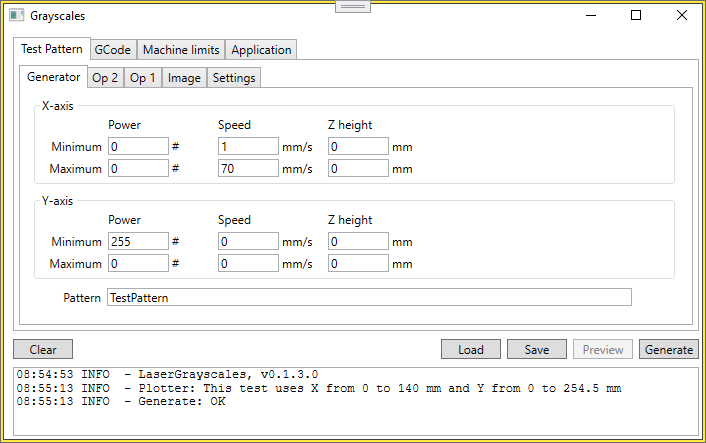
\includegraphics[width=0.8\linewidth]{./images/Grayscales-v0.1.3.png}
\end{figure}

This is the first screen you see when starting up. The top part has a tab selection for `Test Pattern', `GCode', `Machine limits' and `Application'. All these tabs
are explained in the following sections.

At the lower end of the form you see a row of buttons and below that some text.

The text part is functioning as a feed back to tell you what the program is doing and which problems have occurred. It is possible to clean this with the `Clear' button
on the left side above it.

The row of buttons include (from left to righ).
\begin{description}
    \item[Clear] To clear the text part below it.
    \item[Load]  To load a previously saved test pattern, replacing all settings in the `Test Pattern' tab.
    \item[Save]  To save a test pattern, write all settings in `Test Pattern' to file. A file name is suggested and you can change it before writing.
    \item[Preview] To get a preview image of the `Test Pattern' (not yet implemented).
    \item[Generate] To generate a G-Code file from the `Test Pattern' settings and taking in account the limits set for the GCode interpreter and the Machine.
                    The default location for the gcode file is `.\textbackslash{}build\textbackslash{}TestPattern-yyyy-MM-ddTHH.mm.ss.nc'. The name `TestPattern' is
                    taken from the text field `Pattern' in the `Test Pattern', `Generator' sub tab. A timestamp is appended to the name. After successfull generation
                    you are asked where to copy the result to.
\end{description}

\section{The Test Pattern tab}\label{TestPatternTab}
%\begin{figure}[h!]
%    \centering
%    \includegraphics[width=0.8\linewidth]{./images/Generating.png}
%\end{figure}

This is the tab where the layout of a test pattern is configured. It has a sub tab for generator settings, two sub tabs for operations on the image (in this version
the operations are fixed and both for arranging copies of the image), a tab for image settings and a final tab for some general settings. A description of each
sub tab is given below.

The test pattern is rectangle with a number of repeated images in the X and Y direction. Each image has a unique x and y coordinate where the coordinates start
with 1 and ends with a final number. Each image is uniquely identified by its $(x, y)$ coordinates.

Each image is drawn/plotted with a specific setting for speed, laser power and Z height. These three values (known as the `arguments under test') are calculated
based on the $(x, y)$ coordinates from the image, the values will always be within machine limits, underflow is replaced by the machine minimum value and overflow
is replaced by the machine maximum value.

\subsection{The Generator sub tab}\label{TestPatternGeneratorTab}
\begin{figure}[h!]
    \centering
    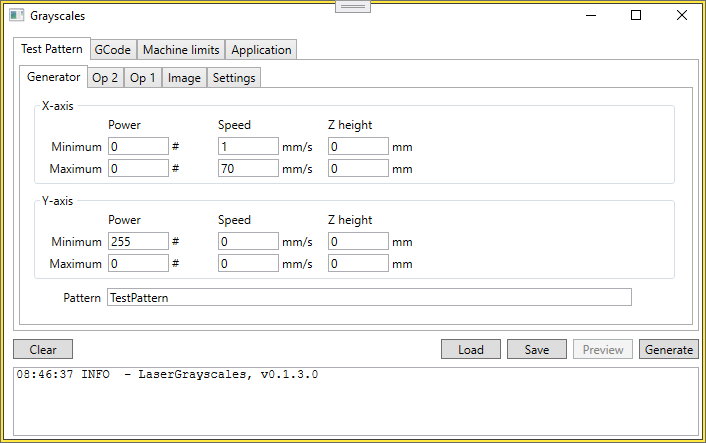
\includegraphics[width=0.8\linewidth]{./images/Generator.png}
\end{figure}

The `Generator' sub tab is for setting values that are used for generating the test pattern. It has three parts.

The first two are `X-axis' and `Y-axis' both with identical settings but obviously for a different axis. For each axis a range of settings for the three
`arguments under test' is defined. Values for X axis and Y axis are added together before using it to draw/plot the image.

It is possible to keep a value at a constant for all images, e.g.: to make the Z height constant at value 0 fill in a 0 for minimum and maximum on both the X and Y axis.

It is possible to change a value in one axis direction only, optionally with a fixed offset, e.g.: speed changing from 1 to 70 mm/sec (60 to 4200 mm/min) in the X direction
and with a fixed offset of 0 specified by the Y direction. It is possible to specify an offset in two (equally valid) ways. The first, as in the example before, is using one axis
for the variations and the other axis for the offset. The other way is to use one axis for both the offset and the variation and set the other axis to a constant value of 0, e.g.:
speed changing from 20 to 50 mm/sec with speed minimum set to 20 and speed maximum set to 50 on the X axis and a value of 0 for both speed minimum and speed maximum on the Y axis.

It is also possible to use different scales on both the X axis and the Y axis this will result in a skewed distribution of values used on the images. In the previous examples
all settings for speed in the Y direction for some index $y$ are identical which makes it easier to evaluate and select a good speed setting. With a skewed setting this is no
longer the case. The advantage of a skewed setting is that it is possible to test a setting over a wider range leaving out some less important combinations of `argument under test'
combinations.

The actual value for $(x, y)$ is calculated with the scale settings and the total number of images in the direction. The total number of images in a direction is depending on
settings for repeat in tabs `Op 1' and `Op 2'.
It is possible to specify a `minimum' value that is bigger than the `maximum' value. More correct names are `start value at the beginning of a sequence' and
`end value at the beginning of a sequence'. Given a total repeat number of $N$ in one direction the value used for index $n$ is `$minimum + \frac{n}{N}(maximum - minimum)$'.
See \nameref{PrinciplesOfOperation} for more details.

The field `Pattern' is used as the base name for the test pattern file generated. See also \nameref{StartupScreen}.

\subsection{The Operation 2 and Operation 1 sub tabs}\label{TestPatternOpTab}
\begin{figure}[h!]
    \centering
    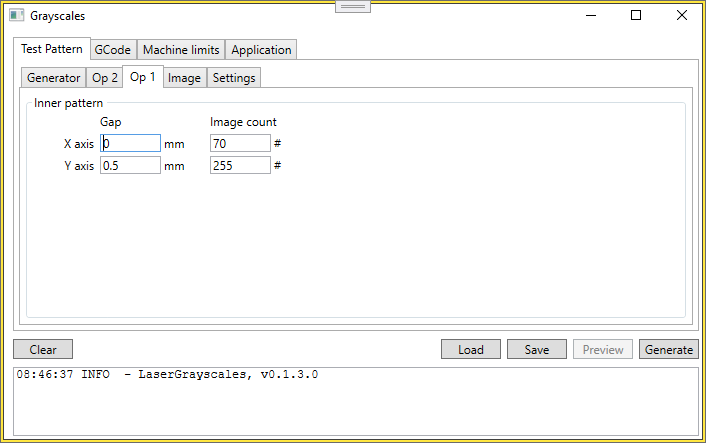
\includegraphics[width=0.8\linewidth]{./images/Operation1.png}
\end{figure}

The `Op 2' and `Op 1' tabs are identical again. Each one specifies a grouping operation in the X and Y direction. `Op 2' is applied before generating and after `Op 1'.
In the same sense `Op 1' is used by `Op 2' and is using `Image'. The name in the tabs used for `Op 2'  is `Outer pattern' en for `Op 1' it is `Inner pattern'.

The repeat pattern specifies a number of copies or `Image count' in the X and Y direction defining a rectangular of images. It also specifies free space or `Gap' in mm
between the repeated images. With the two repeating patterns it is possible to sub divide the final result in groups. This way it is easier for find the actual values
used for `parameters under test'. Note: with the border operation available it will be possible to write an index or value in the final result. This operation is
not yet available.

See \nameref{TestPatternGeneratorTab} for some examples on how to group images. See \nameref{PrinciplesOfOperation} for more details.

\subsection{The Image sub tab}\label{TestPatternImageTab}
\begin{figure}[h!]
    \centering
    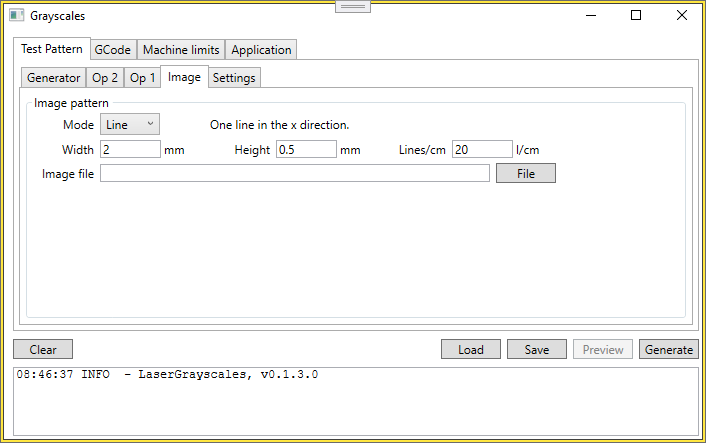
\includegraphics[width=0.8\linewidth]{./images/Image.png}
\end{figure}

In this tab the actual Image to draw in each copy is specified. A few settings are in use for it. An image is always a rectangular shape with a width and a height.
If the rectangle has a filling then the lines per cm is used otherwise it is ignored.

There are four shapes, called `Mode', of images possible.
\begin{description}
    \item[line]   A line at the lower end of the rectangle.
    \item[box]    Four lines, one at each side of the rectangle, no filling in the rectangle.
    \item[square] A box with a lines filling inside running in the x direction.
    \item[card]   A square with an image inside (not yet available).
\end{description}

For normal testing the `Line' mode will give you sufficient information to select the most appropriate settings for `parameters under test' in your application.
Each shape or `Mode' is designed to test some specific properties of the machine and interpreter configuration. See \nameref{PrinciplesOfOperation} for more details.

\subsection{The Settings sub tab}\label{TestPatternSettingsTab}
\begin{figure}[h!]
    \centering
    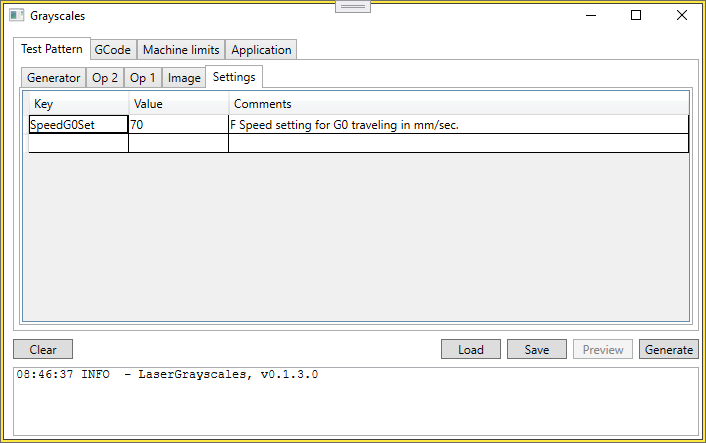
\includegraphics[width=0.8\linewidth]{./images/Settings.png}
\end{figure}

For the test pattern one setting is available. That is the speed (in mm/sec) available for `G0' gcode move actions. This value is limited by the GCode minimum and maximum settings,
see \nameref{GCodeSettingsTab}

\section{The GCode tab}\label{GCodeTab}
\begin{figure}[h!]
    \centering
    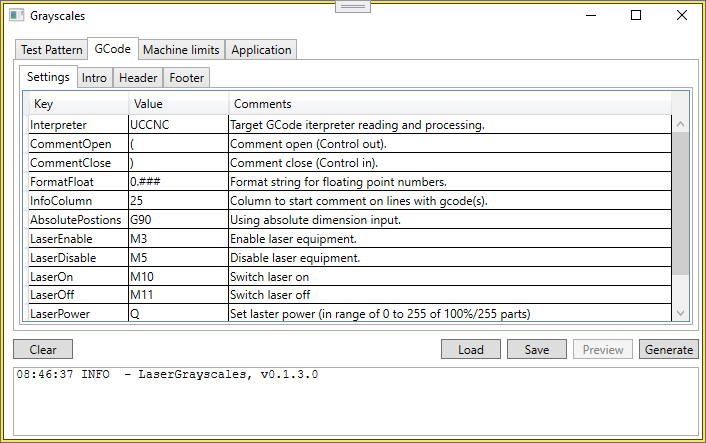
\includegraphics[width=0.8\linewidth]{./images/GCode-Settings.png}
\end{figure}

With the `GCode' tab you can specifiy all gcode specific settings depending on your gcode interpreter, that is `actual code' to use and the Intro/Header/Footer to use with
each test. (The setting for `G0 F speed of travel' is part of the test pattern settings, see \nameref{TestPatternSettingsTab})

\subsection{The Settings sub tab}\label{GCodeSettingsTab}

This sub tab give you full control over the actual GCode that is generated in the script, with one exception. Any GCode that is used in the Intro/Header/Footer sub tabs is
not subject to the settings here. The purpose of the GCode in the configuration should be clear from the `Comments' column. See \nameref{PrinciplesOfOperation} and
\nameref{GCodeAndRs274D} for more information.

\subsection{The Intro, Header and Footer sub tabs}\label{GCodeIntroTab}
\begin{figure}[h!]
    \centering
    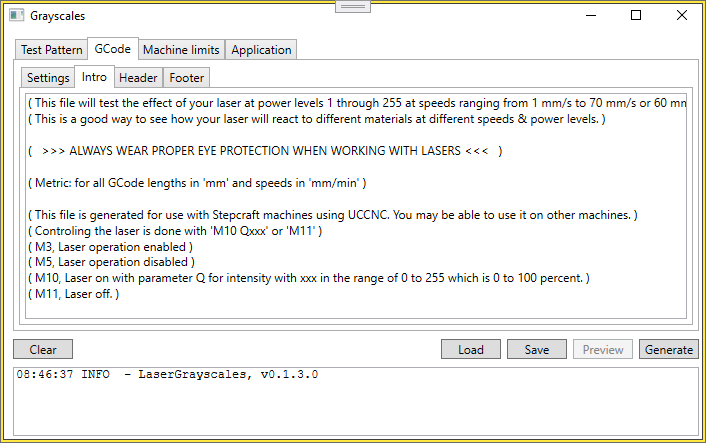
\includegraphics[width=0.8\linewidth]{./images/GCode-Intro.png}
\end{figure}

The tree sub tabs `Into', `Header' and `Footer' are identical. The first is used as an intro in the script generated where the second and last are used
as header and footer for the actions part. Each tab is free text which is copied verbatim into the script. Any GCode used is \emph{not subject to validation}.

\WarningCheckAndTest

\section{The Machine tab}\label{MachineTab}
\begin{figure}[h!]
    \centering
    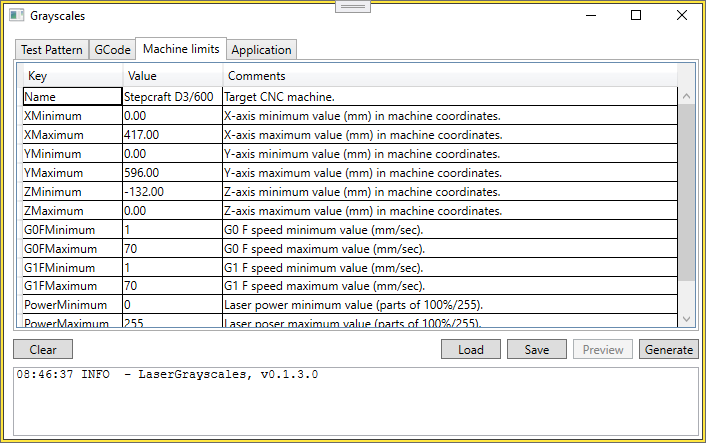
\includegraphics[width=0.8\linewidth]{./images/Machine-limits.png}
\end{figure}

The `Machine limits' tab specifies all minimum and maximum allowed values for variables used while generating a test script. This tab give you the possibility to generate
scripts wit safe and acceptable values for your machine. The purpose of the values in the configuration should be clear from the `Comments' column. See \nameref{PrinciplesOfOperation}
for more information.

\section{The Application tab}\label{ApplicationTab}
\begin{figure}[h!]
    \centering
    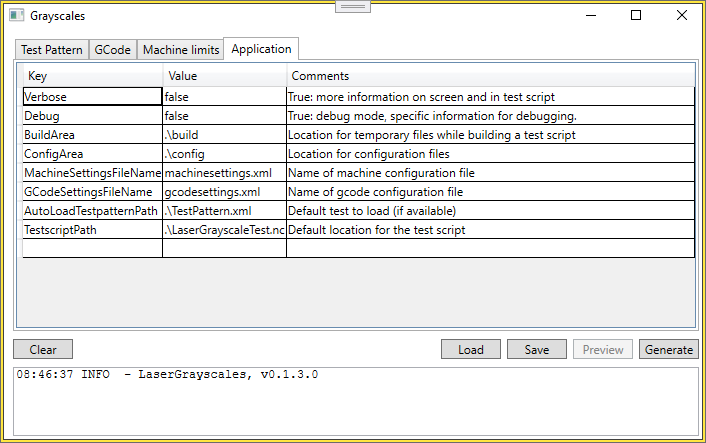
\includegraphics[width=0.8\linewidth]{./images/Application.png}
\end{figure}

The `Application' tab binds a number of items for use in the application. In general it specifies how much information to generate or where to find what kind of information.
Again, the purpose of the values in the configuration should be clear from the `Comments' column.

The application is using two (not necessarily separate) locations for configuration and building. From the configuration area two items are required, if not available
default versions are generated.

This gives you the flexibility to have configurations for several machine (or machine configurations) and several gcode interpreters available. The defaults are for
using a `Stepcraft D3/600' machine. If you for instance create a second configuration file e.g.: for `Stepcraft D2/420' you can use that too. It you use `LinuxCNC' as your
primary gcode interpreter you can use that too. Switching between configurations is now a manual action, you have to edit the `Applications' tab, which will be prone to
typing errors. In some future version a selection screen can come available but this is not yet in the planning.

It is possible to use a template `Test Pattern' that is loaded on each start. This way you are not dependent on default test pattern settings but can configure it for
your most used settings. This file is located independent from the config or build area. In some future version it may be that the last loaded or last generated pattern
will be reloaded. This is not yet available.

